%\renewcommand{\theequation}{\theenumi}
%\begin{enumerate}[label=\arabic*.,ref=\thesubsection.\theenumi]
%\numberwithin{equation}{enumi}
\item Find the equation of a circle with centre \myvec{-3\\2} and radius 4.
\\
\solution 
\input{./solutions/1/chapters/circle/solution2.tex}

\item Find the centre and radius of the circle
\begin{align}
\vec{x}^T\vec{x}+\myvec{8\\10}\vec{x} -8= 0
\end{align}
%
\\
\solution 
%
\begin{align}
    E(X) &= \frac{1}{\sqrt{2\pi}} \int_{-\infty}^{\infty} x e^{-\frac{x^2}{2}}dx\\
    &=0 \quad \brak{ \text{ odd function}}
\end{align}
\begin{align}
    E\brak{X^2}&= \frac{1}{\sqrt{2\pi}}\int_{-\infty}^{\infty} x^2
e^ {-\frac{x^2}{2}} dx \quad \brak{even function}\\
    &= \frac{2}{\sqrt{2\pi}} \int_{0}^{\infty} x^2 e^{-\frac{x^2}{2}} dx\\
    &= \frac{2}{\sqrt{2\pi}}\int_{0}^{\infty}\sqrt{2u}e^{-u} du \quad\brak{Let \frac{x^2}{2}= u}\\
    &= \frac{2}{\sqrt{\pi}} \int_{0}^{\infty} e^{-u} u^{\frac{3}{2}-1} du\\
    &= \frac{2}{\sqrt{\pi}} \Gamma\brak{{\frac{3}{2}}}\\
    &= \frac{1}{\sqrt{\pi}}\Gamma\brak{\frac{1}{2}} \\
    &= 1
\end{align}
where we have used the fact that
\begin{align}
\quad\because \Gamma(n)= (n-1)\Gamma(n-1); \Gamma\brak{\frac{1}{2}}=\sqrt{\pi}
\end{align}
%
Thus, the  variance is
\begin{align}
    \sigma^2 =  E\brak X^2 - E^2\brak X = 1
\end{align}

\item Find the equation of the circle which passes through the points \myvec{2\\-2} and \myvec{3\\4} and whose centre lies on the line 
\begin{align}
\label{eq:4.1.3_line}
\myvec{1 & 1} \vec{x} = 2.
\end{align}
\\
\solution 
%
\begin{align}
    E(X) &= \frac{1}{\sqrt{2\pi}} \int_{-\infty}^{\infty} x e^{-\frac{x^2}{2}}dx\\
    &=0 \quad \brak{ \text{ odd function}}
\end{align}
\begin{align}
    E\brak{X^2}&= \frac{1}{\sqrt{2\pi}}\int_{-\infty}^{\infty} x^2
e^ {-\frac{x^2}{2}} dx \quad \brak{even function}\\
    &= \frac{2}{\sqrt{2\pi}} \int_{0}^{\infty} x^2 e^{-\frac{x^2}{2}} dx\\
    &= \frac{2}{\sqrt{2\pi}}\int_{0}^{\infty}\sqrt{2u}e^{-u} du \quad\brak{Let \frac{x^2}{2}= u}\\
    &= \frac{2}{\sqrt{\pi}} \int_{0}^{\infty} e^{-u} u^{\frac{3}{2}-1} du\\
    &= \frac{2}{\sqrt{\pi}} \Gamma\brak{{\frac{3}{2}}}\\
    &= \frac{1}{\sqrt{\pi}}\Gamma\brak{\frac{1}{2}} \\
    &= 1
\end{align}
where we have used the fact that
\begin{align}
\quad\because \Gamma(n)= (n-1)\Gamma(n-1); \Gamma\brak{\frac{1}{2}}=\sqrt{\pi}
\end{align}
%
Thus, the  variance is
\begin{align}
    \sigma^2 =  E\brak X^2 - E^2\brak X = 1
\end{align}

\item Find the area enclosed by the circle $\norm{\vec{x}} = a$
%
\\
\solution The area is $2\pi a^2$.
%
\item Find the area of the region in the first quadrant enclosed by the x-axis, the line $\myvec{1 & -1}\vec{x} = 0$, and the circle $\norm{\vec{x}} = 1$.
%
\\
\solution 
%
\begin{align}
    E(X) &= \frac{1}{\sqrt{2\pi}} \int_{-\infty}^{\infty} x e^{-\frac{x^2}{2}}dx\\
    &=0 \quad \brak{ \text{ odd function}}
\end{align}
\begin{align}
    E\brak{X^2}&= \frac{1}{\sqrt{2\pi}}\int_{-\infty}^{\infty} x^2
e^ {-\frac{x^2}{2}} dx \quad \brak{even function}\\
    &= \frac{2}{\sqrt{2\pi}} \int_{0}^{\infty} x^2 e^{-\frac{x^2}{2}} dx\\
    &= \frac{2}{\sqrt{2\pi}}\int_{0}^{\infty}\sqrt{2u}e^{-u} du \quad\brak{Let \frac{x^2}{2}= u}\\
    &= \frac{2}{\sqrt{\pi}} \int_{0}^{\infty} e^{-u} u^{\frac{3}{2}-1} du\\
    &= \frac{2}{\sqrt{\pi}} \Gamma\brak{{\frac{3}{2}}}\\
    &= \frac{1}{\sqrt{\pi}}\Gamma\brak{\frac{1}{2}} \\
    &= 1
\end{align}
where we have used the fact that
\begin{align}
\quad\because \Gamma(n)= (n-1)\Gamma(n-1); \Gamma\brak{\frac{1}{2}}=\sqrt{\pi}
\end{align}
%
Thus, the  variance is
\begin{align}
    \sigma^2 =  E\brak X^2 - E^2\brak X = 1
\end{align}

%
\item Find the area of the region enclosed between the two circles: $\vec{x}^T\vec{x} = 4$ and $\norm{\vec{x}-\myvec{2\\0}} = 2$.
%
\item Find the coordinates of a point $\vec{A}$, where $AB$ is the diameter of a circle whose centre is \myvec{2,-3} and $\vec{B} = \myvec{1\\4}$.
\\
\solution 
%
\begin{align}
    E(X) &= \frac{1}{\sqrt{2\pi}} \int_{-\infty}^{\infty} x e^{-\frac{x^2}{2}}dx\\
    &=0 \quad \brak{ \text{ odd function}}
\end{align}
\begin{align}
    E\brak{X^2}&= \frac{1}{\sqrt{2\pi}}\int_{-\infty}^{\infty} x^2
e^ {-\frac{x^2}{2}} dx \quad \brak{even function}\\
    &= \frac{2}{\sqrt{2\pi}} \int_{0}^{\infty} x^2 e^{-\frac{x^2}{2}} dx\\
    &= \frac{2}{\sqrt{2\pi}}\int_{0}^{\infty}\sqrt{2u}e^{-u} du \quad\brak{Let \frac{x^2}{2}= u}\\
    &= \frac{2}{\sqrt{\pi}} \int_{0}^{\infty} e^{-u} u^{\frac{3}{2}-1} du\\
    &= \frac{2}{\sqrt{\pi}} \Gamma\brak{{\frac{3}{2}}}\\
    &= \frac{1}{\sqrt{\pi}}\Gamma\brak{\frac{1}{2}} \\
    &= 1
\end{align}
where we have used the fact that
\begin{align}
\quad\because \Gamma(n)= (n-1)\Gamma(n-1); \Gamma\brak{\frac{1}{2}}=\sqrt{\pi}
\end{align}
%
Thus, the  variance is
\begin{align}
    \sigma^2 =  E\brak X^2 - E^2\brak X = 1
\end{align}

\item Find the centre $O$ of a circle passing through the points \myvec{6\\-6}, \myvec{3\\-7} and  \myvec{3\\3}.
\solution 
%
\begin{align}
    E(X) &= \frac{1}{\sqrt{2\pi}} \int_{-\infty}^{\infty} x e^{-\frac{x^2}{2}}dx\\
    &=0 \quad \brak{ \text{ odd function}}
\end{align}
\begin{align}
    E\brak{X^2}&= \frac{1}{\sqrt{2\pi}}\int_{-\infty}^{\infty} x^2
e^ {-\frac{x^2}{2}} dx \quad \brak{even function}\\
    &= \frac{2}{\sqrt{2\pi}} \int_{0}^{\infty} x^2 e^{-\frac{x^2}{2}} dx\\
    &= \frac{2}{\sqrt{2\pi}}\int_{0}^{\infty}\sqrt{2u}e^{-u} du \quad\brak{Let \frac{x^2}{2}= u}\\
    &= \frac{2}{\sqrt{\pi}} \int_{0}^{\infty} e^{-u} u^{\frac{3}{2}-1} du\\
    &= \frac{2}{\sqrt{\pi}} \Gamma\brak{{\frac{3}{2}}}\\
    &= \frac{1}{\sqrt{\pi}}\Gamma\brak{\frac{1}{2}} \\
    &= 1
\end{align}
where we have used the fact that
\begin{align}
\quad\because \Gamma(n)= (n-1)\Gamma(n-1); \Gamma\brak{\frac{1}{2}}=\sqrt{\pi}
\end{align}
%
Thus, the  variance is
\begin{align}
    \sigma^2 =  E\brak X^2 - E^2\brak X = 1
\end{align}

\item Sketch the circles with 
\begin{enumerate}
\item centre \myvec{0\\2} and radius 2
\item centre \myvec{-2\\32} and radius 4
\item centre $\myvec{\frac{1}{2}\\ \frac{1}{4}}$ and radius $\frac{1}{12}$.
\item centre \myvec{1\\1} and radius $\sqrt{2}$.
\item centre \myvec{-a\\-b} and radius $\sqrt{a^2-b^2}$.
\end{enumerate}
\solution 
%
\begin{align}
    E(X) &= \frac{1}{\sqrt{2\pi}} \int_{-\infty}^{\infty} x e^{-\frac{x^2}{2}}dx\\
    &=0 \quad \brak{ \text{ odd function}}
\end{align}
\begin{align}
    E\brak{X^2}&= \frac{1}{\sqrt{2\pi}}\int_{-\infty}^{\infty} x^2
e^ {-\frac{x^2}{2}} dx \quad \brak{even function}\\
    &= \frac{2}{\sqrt{2\pi}} \int_{0}^{\infty} x^2 e^{-\frac{x^2}{2}} dx\\
    &= \frac{2}{\sqrt{2\pi}}\int_{0}^{\infty}\sqrt{2u}e^{-u} du \quad\brak{Let \frac{x^2}{2}= u}\\
    &= \frac{2}{\sqrt{\pi}} \int_{0}^{\infty} e^{-u} u^{\frac{3}{2}-1} du\\
    &= \frac{2}{\sqrt{\pi}} \Gamma\brak{{\frac{3}{2}}}\\
    &= \frac{1}{\sqrt{\pi}}\Gamma\brak{\frac{1}{2}} \\
    &= 1
\end{align}
where we have used the fact that
\begin{align}
\quad\because \Gamma(n)= (n-1)\Gamma(n-1); \Gamma\brak{\frac{1}{2}}=\sqrt{\pi}
\end{align}
%
Thus, the  variance is
\begin{align}
    \sigma^2 =  E\brak X^2 - E^2\brak X = 1
\end{align}

\item  Does the point \myvec{–2.5\\ 3.5} lie inside, outside or on the circle $\vec{x}^T\vec{x} = 25$?
\\
\solution 
\input{./solutions/4/chapters/circle/solution2.tex}
\item Sketch the circles with equation
\begin{enumerate}
\item $\norm{\vec{x}-\myvec{5\\-3}}^2 = 36$
\item $\vec{x}^T\vec{x}-\myvec{4\\8}\vec{x} -45= 0$
\item $\vec{x}^T\vec{x}-\myvec{8\\-10}\vec{x} -12= 0$
\item $2\vec{x}^T\vec{x}-\myvec{1\\0}\vec{x} = 0$
\end{enumerate}
\solution 
\input{./solutions/5/chapters/circle/docq18.tex}
\item Find the equation of the circle passing through the points \myvec{4\\1} and \myvec{6\\5} and whose centre is on the line $\myvec{4 & 1}\vec{x} = 16$.
\\
\solution 
%
\begin{align}
    E(X) &= \frac{1}{\sqrt{2\pi}} \int_{-\infty}^{\infty} x e^{-\frac{x^2}{2}}dx\\
    &=0 \quad \brak{ \text{ odd function}}
\end{align}
\begin{align}
    E\brak{X^2}&= \frac{1}{\sqrt{2\pi}}\int_{-\infty}^{\infty} x^2
e^ {-\frac{x^2}{2}} dx \quad \brak{even function}\\
    &= \frac{2}{\sqrt{2\pi}} \int_{0}^{\infty} x^2 e^{-\frac{x^2}{2}} dx\\
    &= \frac{2}{\sqrt{2\pi}}\int_{0}^{\infty}\sqrt{2u}e^{-u} du \quad\brak{Let \frac{x^2}{2}= u}\\
    &= \frac{2}{\sqrt{\pi}} \int_{0}^{\infty} e^{-u} u^{\frac{3}{2}-1} du\\
    &= \frac{2}{\sqrt{\pi}} \Gamma\brak{{\frac{3}{2}}}\\
    &= \frac{1}{\sqrt{\pi}}\Gamma\brak{\frac{1}{2}} \\
    &= 1
\end{align}
where we have used the fact that
\begin{align}
\quad\because \Gamma(n)= (n-1)\Gamma(n-1); \Gamma\brak{\frac{1}{2}}=\sqrt{\pi}
\end{align}
%
Thus, the  variance is
\begin{align}
    \sigma^2 =  E\brak X^2 - E^2\brak X = 1
\end{align}

\item Find the equation of the circle passing through the points $\vec{P} =\myvec{2\\3}$ and $\vec{Q} = \myvec{–1\\1}$ and whose centre is on the line $\myvec{1 & -3}\vec{x} = 11$.
\solution 
%
\begin{align}
    E(X) &= \frac{1}{\sqrt{2\pi}} \int_{-\infty}^{\infty} x e^{-\frac{x^2}{2}}dx\\
    &=0 \quad \brak{ \text{ odd function}}
\end{align}
\begin{align}
    E\brak{X^2}&= \frac{1}{\sqrt{2\pi}}\int_{-\infty}^{\infty} x^2
e^ {-\frac{x^2}{2}} dx \quad \brak{even function}\\
    &= \frac{2}{\sqrt{2\pi}} \int_{0}^{\infty} x^2 e^{-\frac{x^2}{2}} dx\\
    &= \frac{2}{\sqrt{2\pi}}\int_{0}^{\infty}\sqrt{2u}e^{-u} du \quad\brak{Let \frac{x^2}{2}= u}\\
    &= \frac{2}{\sqrt{\pi}} \int_{0}^{\infty} e^{-u} u^{\frac{3}{2}-1} du\\
    &= \frac{2}{\sqrt{\pi}} \Gamma\brak{{\frac{3}{2}}}\\
    &= \frac{1}{\sqrt{\pi}}\Gamma\brak{\frac{1}{2}} \\
    &= 1
\end{align}
where we have used the fact that
\begin{align}
\quad\because \Gamma(n)= (n-1)\Gamma(n-1); \Gamma\brak{\frac{1}{2}}=\sqrt{\pi}
\end{align}
%
Thus, the  variance is
\begin{align}
    \sigma^2 =  E\brak X^2 - E^2\brak X = 1
\end{align}

\item Find the equation of the circle with radius 5 whose centre lies on x-axis and passes through the point \myvec{2\\3}.
\\
\solution
Let $\vec{O}$ be the centre and $r$ be the radius of the given circle.
\\
$\therefore$
\begin{align}
    \label{eq:quad_form/2/1}
    \begin{split}
\vec{O} &= \myvec{p\\0}
\\
r &= 5
    \end{split}
\end{align}

The general equation of a circle is given by 
\begin{align}
\vec{x}^T\vec{x} - 2\vec{O}^T\vec{x} + \norm{\vec{O}}^2 -r^2 = 0
\end{align}
which, upon substitution from \eqref{eq:quad_form/2/1} yields
\begin{align}
\vec{x}^T\vec{x} - 2\myvec{p & 0}\vec{x} + p^2 - 25 = 0
\end{align}
$\because$
Point $\vec{A}$=\myvec{2\\3} lies on the circle, 
%
\begin{align}
\myvec{2 & 3}\myvec{2\\3} - 2\myvec{p & 0}\myvec{2\\3} + p^2 -25 &=0
\\
\implies p^2 - 4p - 12 &=0
\\
\implies p &=6 
\text{ or } -2
\end{align}

Hence,the possible equations of the circle are
\begin{align}
\vec{x}^T\vec{x} - 2\myvec{6 & 0}\vec{x} + 11 &= 0 \label{quad_form/2/1eq:1}
\\
\text{or}, \vec{x}^T\vec{x} - 2\myvec{-2 & 0}\vec{x} - 21 &= 0 \label{quad_form/2/1eq:2}
\end{align}

which are plotted in Fig. \ref{quad_form/2/1fig:circle}	


\begin{figure}[!ht]
\centering
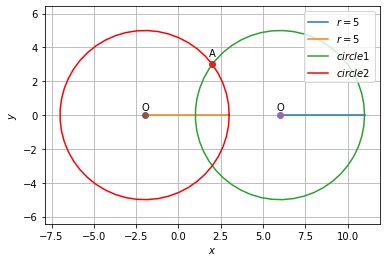
\includegraphics[width=\columnwidth]{solutions/su2021/2/1/Figure5.png}
\caption{Circles with centres (6,0) and (-2,0) respectively }
\label{quad_form/2/1fig:circle}	
\end{figure}




%\end{enumerate}
